\chapter{ITIL V3 \& Vertiefung IT-Betriebsprozesse}

\section{Sie kennen und verstehen die wichtigsten IT-Betriebsprozesse aus ITIL V3 und deren Bedeutung für das Unternehmen.}

\subsection{Service Strategy}

Die Phase Service Strategy beinhaltet folgende Prozesse:

\begin{description}
	\item[Strategy Management for IT-Services:] Dieser Prozess beschreibt, wie die Business-Strategie und die IT-Strategie gestaltet, etabliert und durchgesetzt werden können. In diesen Strategien wird festgelegt, wie ein Service Provider die Geschäftsprozesse eines Unternehmens unterstützen und so die die Ergebnisse des Business positiv beeinflussen kann.
	\item[Service Portfolio Management:] Das Service Portfolio Management beschreibt die Services im Business-Kontext, also bezogen auf den Nutzen für die Kunden, und liefert die Basis für den Servicekatalog.
	\item[Financial Management:] Das Financial Management unterstützt Unternehmen dabei, den Ressourceneinsatz für die Erreichung der Unternehmensziele sinnvoll und entsprechend den vorhandenen Mitteln und Möglichkeiten zu steuern.
	\item[Demand Management:] Das Demand Management versucht den Bedarf des Kunden im Detail zu verstehen und Voraussagen zu treffen.
	\item[Business Relationship Management:] Das Business Relationship Management versucht eine gute Beziehung zwischen Service Provider und dem Kunden zu etablieren.
\end{description}

\subsection{Service Design}

Die Phase Service Design beinhaltet folgende Prozesse:

\begin{description}
	\item[Design Coordination:] Die Design Coordination sollte die Aktivitäten während der gesamten Design-Phase zentral koordinieren.
	\item[Service Catalogue Management:] Das Service Catalogue Management ist verantwortlich für die Bereitstellung, Pflege und Vollständigkeit des Servicekatalogs sowie für die Kommunikation der Inhalte	sowohl an den Kunden als auch an alle Beteiligten beim Service Provider selbst.
	\item[Service Level Management:] Das Service Level Management sammelt die Anforderungen des Business und erstellt aufgrund dessen Service Level Agreements (SLA).
	\item[Availability Management:] Das Availability Management versucht die Verfügbarkeit aktueller und zukünftiger Services an die Anforderungen des Business anzupassen.
	\item[Capacity Management:] Das Capacity Management versucht ausreichend Ressourcen zur Verfügung zu stellen und Überkapazitäten zu meiden.
	\item[Information Security Management:] Das Information Security Management richtet die IT-Sicherheit an den Anforderungen des Business aus.
	\item[IT Service Continuity Management:] Das Continuity Management stellt sicher das der Kunde im Katastrophenfall mit einem definierten Minimum an Services arbeiten kann. Auch die Wiederherstellung des Betriebs gehört dazu.
	\item[Supplier Management:] Das Supplier Management steuert und überprüft die externen Lieferanten gemäss den vereinbarten Anforderungen.
\end{description}

\subsection{Service Transition}

Die Phase Service Transition beinhaltet folgende Prozesse:
\begin{description}
	\item[Transition Planning \& Support:] Der Transition Support unterstützt die Transition-Teams bei der Überführung von Services in den Betrieb.
	\item[Change Management:] Das Change Management kontrolliert alle Veränderungen an vorhandenen Services, das Hinzufügen
	neuer Services und die Ausserbetriebnahme von Services.
	\item[Service Asset \& Configuration Management:] Das Configuration Management stellt aktuelle und konsistente Konfigurationen der IT-Infrastruktur zur Verfügung.
	\item[Release \& Deployment Management:] Das Release Management sorgt für eine reibungslose Integration neuer Service-Releases in die Zielumgebung gemäss einem Zeitplan.
	\item[Service Validation \& Testing:] Das Service Validation \& Testing prüft ob die neuen oder veränderten Services die Anforderungen erfüllen.
	\item[Change Evaluation:] Der Change-Evaluation-Prozess dient dazu, festzustellen, ob ein neuer oder veränderter Service die erwartete Performance liefert und ob die Kosten diesen Nutzen rechtfertigen.
	\item[Knowledge Management:] Das Knowledge Management stellt die richtigen Informationen am richtigen
	Ort für die richtigen Personen zur richtigen Zeit zur Verfügung.
\end{description}
In der Praxis sind nur Change, Configuration, Deployment und Testing relevant.

\subsection{Service Operation}

Die Phase Service Strategy beinhaltet folgende Prozesse:
\begin{description}
	\item[Event Management (Monitoring):] Das Event Management hält auftretende Ereignisse in der IT-Infrastruktur fest und leitet entsprechende Massnahmen ein.
	\item[Incident Management:] Das Incident Management befasst sich mit allen Ereignissen, die einen Service stören oder beeinflussen können.
	\item[Problem Management:] Das Problem Management versucht präventiv Incidents zu vermeiden oder deren Auswirkung zu minimieren.
	\item[Request Fulfilment:] Das Request Fulfilment befasst sich mit dem Management von Anwenderanfragen.
	\item[Access Management:] Das Access Management ist verantwortlich für die Verwaltung der Zugriffsrechte.
\end{description}
Neben den oben genannten Prozessen sind im Service Operation auch Funktionen beschrieben. Funktionen sind auf Personen oder Organisationseinheiten bezogen, welche bestimmte Prozesse oder Aktivitäten ausführen. Die Funktionen im Überblick:
\begin{itemize}
	\item Service Desk
	\item Technical Management
    \item IT-Operations Management
	\item Application Management
\end{itemize}

\subsection{Continual Service Improvement}
\begin{itemize}
	\item Grundlegende Unterstützung und Anleitung zur Erzeugung und Erhaltung von Mehrwert für den Kunden durch die kontinuierliche Verbesserung von Service Design, Service Transition und Services Operation.
	\item Es werden Methoden des Qualitätsmanagements, Change Management und Capability Improvement kombiniert.
\end{itemize}


\section{Sie kennen folgende ITIL-Prozesse vertieft:} 

\subsection{Service Level Mgmt.}

\subsubsection{Ziele}

Ziel des Service Level Management ist die Definition, Dokumentation und Vereinbarung von Service Level Agreements (SLA). Ein SLA sollte so vereinbart werden, dass er den Erwartungen der Kunden und auch den Fähigkeiten des Service Providers gerecht wird. Zusätzlich sollten auch Messungen vereinbart werden damit die Servicequalität überprüft werden kann. Diese Massnahmen führen zu einer besseren Beziehung zwischen Kunden und Service Provider. Detailliertere Informationen findet man im Abschnitt \ref{sec:service-level-management}.

\subsubsection{Begriffe}

\begin{description}
	\item[Service Packages:] Ein Service Package ist aus mehreren Services zusammengesetzt und beschreibt die angebotenen Leistungen für den Kunden.
\end{description}

\subsubsection{Aktivitäten}

\begin{description}
	\item[Vereinbarungen zur Serviceerbringung:] Bei dieser Aktivität werden die Kundenanforderungen in SLR gesammelt und basierend darauf ein SLA erstellt. Je besser der SLA den Kundenanforderungen entsprechen desto grösser ist die Kundenzufriedenheit. Der Service Level Manager übersetzt zwischen Business und IT-Fachbereich und erstellt darauf aufbauend OLA mit den IT-Fachbereichen. Externe Leistungen werden über Contracts bezogen.
	\item[Service Review:] Für eine gleich bleibende Servicequalität müssen die getroffenen Vereinbarungen kontinuierlich
	überprüft und bei Bedarf angepasst werden. Deshalb führt der Service Level Manager regelmässig Reviews durch, um die Services zu überprüfen.
	\item[Messen und Berichten:] Damit die Kunden den Nutzen der Services erkennen und überprüfen können, ob der Service
	Provider die Services wie vereinbart liefert, ist ein regelmässiges Reporting unverzichtbar. Die im SLA vereinbarten Messungen werden in dieser Aktivität an den Kunden weitergeleitet.
	\item[Kundenzufriedenheit sicherstellen und erhöhen:] Die Zufriedenheit der Anwender auf Kundenseite wirkt sich sehr stark darauf aus, wie der Kunde den Service Provider wahrnimmt. Deshalb wird in dieser Aktivität die Zufriedenheit des Kunden durch Befragung ermittelt (Nicht übertreiben!)
\end{description}

\subsubsection{Rollen}

\begin{description}
	\item[Service Level Manager:] Der Service Level Manager muss dafür sorgen das die Prozessaktivitäten von den Prozessbeteiligten ausgeführt werden. Zusätzlich identifiziert er die Kundenanforderungen (SLR) und gestaltet daraus Servicevereinbarungen (SLA).
	\item[IT-Planer:] Der IT-Planer ist verantwortlich für die Erstellung und Koordination von IT-Plänen zur Umsetzung der Geschäftsanforderungen. Der IT-Planer hat also einen wesentlichen Einfluss auf die Gestaltung der SLA.
\end{description}

\subsubsection{KPI's}

\begin{itemize}
	\item Anteil nicht erfüllter SLA
	\item Prozentuale Verbesserung der Kundenzufriedenheit durch Zufriedenheitsanalysen
	\item Anteil der Services mit SLA
\end{itemize}

\subsection{IT Service Continuity Mgmt.}

\subsubsection{Ziele}

In den meisten Unternehmen ist bereits ein Business Continuity Management vorhanden. Das ist ein unternehmensweiter Management-Ansatz um kritische Geschäftsfunktionen aufrecht zu erhalten. Das IT Service Continuity Management ist der IT-spezifische Bestandteil des BCM. ITSCM stellt sicher, dass der Kunde im Katastrophenfall mit einem definierten Minimum an Services arbeiten kann. Zudem gilt es, die Fähigkeiten und Ressourcen so zu gestalten, dass die Services zur Unterstützung der Geschäftsprozesse nach einer Katastrophe in der vorgegebenen Zeit wiederhergestellt werden können.

\subsubsection{Begriffe}

\begin{description}
	\item[IT-Service Continuity Plan:] Der ITSCM-Plan ist Bestandteil des Business Continuity Plans und erfüllt dessen Vorgaben. Im Plan sind die Schritte zur Wiederherstellung beschrieben, wann der Plan aktiv wird und die Zuständigkeit und Rollen sind definiert.
	\item[Störung:] Eine Störung ist ein Ereignis welches zu einer Einschränkung oder zu einem Ausfall eines Services führt. Eine Störung wird im Incident Management behandelt. Treten mehrere Störungen mit signifikanter Auswirkung auf die Geschäftsprozesse ein entsteht eine Krise.
	\item[Krise:] Eine Krise ist eine Bedrohungssituation, welche kritische Entscheidungen erfordert, die mit den ordentlichen Führungsmitteln und Entscheidungskompetenzen nicht bewältigt werden können. Wird in einem Krisenmanagement behandelt.
\end{description}

\subsubsection{Aktivitäten}

\begin{description}
	\item[Initiierung:] In der Initiierungsphase wird der Scope des ITSCM festgelegt. Der Umfang wird aus den \emph{vitalen Business Funktionen} abgeleitet, welche dem BCM entnommen wurden. Nachdem der Umfang definiert wurde müssen entsprechende Ressourcen bereitgestellt werden und Verantwortlichkeiten zugeteilt werden.
	\item[Anforderungen und Strategie:] In einem ersten Schritt wird mittels einer \emph{Business-Impact-Analysis} die geschäftskritischen Prozesse erkannt und die Auswirkungen eines Ausfalls beschrieben. Danach werden mit einem \emph{Risk Assessment} die Risiken eines Prozesses bewertet und einer Risikostufe zugeteilt. Abschliessend legt die \emph{IT-Service Continuity Strategie} fest, mit welchen Recovery-Optionen (manueller Workaround, sofortige Wiederherstellung usw.) ein Prozess wiederhergestellt werden soll.
	\item[Implementierung:] In dieser Phase wird die geplante Strategie umgesetzt. Es wird ein ITSCM-Plan erstellt und im Unternehmen kommuniziert. Bei Bedarf können weitere Pläne erstellt werden (z.B. Notfall-Kommunikationsplan). Nachdem alle Massnahmen implementiert wurden sollte unbedingt ein initialer Test durchgeführt werden, um zu überprüfen ob die Massnahmen klappen.
	\item[Operativer Betrieb:] In der Phase Operativer Betrieb wird das ITSCM im Unternehmen dauerhaft etabliert. Das gelingt nur wenn die Wiederherstellungsprozesse regelmässig geübt und Reviews durchgeführt werden. Auch das Change Management muss evtl. Änderungen mitteilen damit das ITSCM entsprechend angepasst werden kann.
\end{description}

\subsubsection{Rollen}

\begin{description}
	\item[IT-Service Continuity Manager:] Er ist verantwortlich für den Prozess und entwickelt die Continuity Strategie und Plan. Bei grösseren Changes passt er auch die betroffenen Dokumente an.
	\item[Executive Board:] Im Executive Board befinden sich auch Mitglieder des Senior Management welche das ITSCM auslösen.
	\item[Desaster-Manager:] Verantwortliche Person und sein Führungsgremium unterhalb des Executive Board.
	\item[Wiederherstellungsteams:] Führen die vereinbarten Massnahmen aus.
\end{description}

\subsubsection{KPI's}

\begin{itemize}
	\item Planmässigkeit der durchgeführten Tests
	\item Anzahl der in Tests festgestellten Mängel
\end{itemize}

\subsection{Service Asset \& Configuration Mgmt.}

\subsubsection{Ziele}

Service Asset \& Configuration Management (SACM) hat das Ziel, aktuelle und konsistente Informationen zur Konfiguration der IT-Infrastruktur und allen zur Service-Erbringung benötigten Komponenten bereitzustellen. Damit die Informationen konsistent und aktuell bleiben müssen regelmässige Überprüfungen durchgeführt werden. Es sollte auch wirklich nur die benötigten Informationen festgehalten werden, damit die Informationen relevant bleiben.

\subsubsection{Begriffe}

\begin{description}
	\item[Configuration Item (CI):] Ein CI ist irgendein Objekt (Hardware, Software, SLA's, Gebäude usw.) das unter der Kontrolle des Configuration Management steht oder stehen wird. Ein CI unterliegt dem Change Management und darf nicht ohne formalen Antrag einfach geändert werden.
	\item[Configuration Model:] Die Beziehungen zwischen verschiedenen CI werden in einem Configuration Model abgebildet. Diese Information wird z.B. vom Change Management oder dem Availability Management verwendet.
	\item[Definitive Media Library (DML):] In der DML werden alle geprüften und freigegebenen CI-Medien aufbewahrt. Als Beispiel können CDs in einem feuerfesten Safe aufbewahrt werden.
	\item[Configuration Management System (CMS):] Im CMS werdn sämtliche Daten der CI zentral gesammelt und verwaltet. Die Daten sollten wenn möglich automatisiert erfasst werden.
	\item[Configuration Baseline:] Die Baseline ist eine aufgezeichnete Konfiguration eines Produktes zu einem bestimmten Zeitpunkt. Sie wird verwendet um Änderungen durchzuführen und bei einem Fehlschlag wieder auf diese Ausgangskonfiguration zurückzugehen.
	\item[Asset Management:] Das Anlagevermögen eins Unternehmens setzt sich aus Assets zusammen, die einen finanziellen Wert haben und genutzt werden können, um Produkte oder Services zu erstellen. Meistens sind dieser Prozesse (Labeln der Assets usw.) bereits etabliert.
\end{description}

\subsubsection{Aktivitäten}

\begin{description}
	\item[Management und Planung:] In dieser Aktivität werden die Rahmenbedingungen und der Scope des SACM festgelegt. Also die verwendeten Tools, die Prozesse und Rollen.
	\item[Konfigurationsidentifizierung:] Zunächst wird definiert nach welchen Kriterien ein CI identifiziert und gruppiert wird. Sind diese Kriterien festgelegt müssen die CI identifiziert und eingeordnet werden. Wichtig ist hier die richtige Erfassungstiefe, denn zu viele Details führen zu einer schwer zu pflegenden Datenmenge.
	\item[Konfigurationssteuerung:] Alle CI sollen während ihres kompletten Lifecycles einer Kontrolle unterliegen. Jede Änderung muss dokumentiert und das CI aktualisiert werden. Wird das nicht gemacht gibt es eine grosse Abweichung zwischen Dokumentation und Realität.
	\item[Statusnachweis und Reporting:] Ein CI kann verschiedene Status (In Planung, In Betrieb usw.) annehmen. In dieser Aktivität wird definiert wie ein Statuswechsel passiert und wer dafür die Verantwortung trägt. Zusätzlich sollten von jedem CI Reports zur Verfügung stehen.
	\item[Verifizieren und Auditieren:] Eine regelmässige aber auch ungeplante Überprüfungen der Informationen eines CI stellen sicher das die Daten der Realität entsprechen. Diese Tätigkeit kann durch Stichproben oder auch automatisiert durchgeführt werden.
\end{description}

\subsubsection{Rollen}

\begin{description}
	\item[Configuration Manager:] Der Configuration Manager ist verantwortlich für die Vereinbarung von Scope und Zielen mit dem IT-Management und für die Definition sowie die Einhaltung der Aktivitäten im Configuration-Management-Prozess.
	\item[Configuration Administrator:] Diese Rolle sorgt für die Identifizierung und die Pflege der CI.
	\item[CMS/Tools Administrator:] Der CMS Administrator ist verantwortlich für die Funktionsfähigkeit der eingesetzten Tools für das Configuration Management.
\end{description}

\subsubsection{KPI's}

\begin{itemize}
	\item Anzahl Abweichungen bei Audits
	\item Anteil erfolgloser Changes aufgrund fehlender oder falscher Information aus dem CMS
	\item Quote genutzter Lizenzen in Bezug zu gekauften Lizenzen
\end{itemize}

\subsection{Monitoring \& Event Mgmt.}

Dieser Prozess wird im Abschnitt \ref{sec:monitoring} ausführlich beschrieben.

\subsection{Incident-Mgmt.}

\subsubsection{Ziele}

Das Incident Management befasst sich mit allen Ereignissen, die einen Service stören oder beeinflussen können, und ist verantwortlich für den gesamten Lebenszyklus aller Incidents. Wichtigstes Ziel des Incident Management ist die schnellstmögliche Wiederherstellung des SLA-konformen Servicebetriebs und die Minimierung negativer Auswirkungen auf die Geschäftsprozesse. Um eine schnelle Wiederherstellung zu ermöglichen sollten die Incidents priorisiert werden, je nachdem wie die Geschäftsprozesse beeinflusst werden.

\subsubsection{Begriffe}

\begin{description}
	\item[Incident:] Ein Incident ist eine ungeplante Unterbrechung oder Reduktion der Qualität eines IT-Service. Auch Ausfälle welche keinen direkte Auswirkung auf den Service haben (z.B. Ausfall RAID-Festplatte) sind ein Incident.
	\item[Workaround:] Ein Workaround ist eine Massnahme zur Reduzierung der Auswirkung eines Incidents, solange keine endgültige Lösung bereitsteht. Workarounds werden meist in einer Knowledge-Datenbank festgehalten.
	\item[Timescales:] Für jeden Bearbeitungsschritt eines Incidents wird im SLA ein Zeitfenster definiert welche vom OLA oder Contract eingehalten werden muss.
	\item[Incident Models:] Incident Models sind vordefinierte Abläufe um auf ähnliche Incidents zu reagieren.
	\item[Major Incidents:] Ein Major Incident hat eine grosse Auswirkung auf die Geschäftsprozesse und muss dementsprechend speziell gehandhabt werden. Im SLA sollte Kriterien für einen Major Incident definiert werden.
\end{description}

\subsubsection{Aktivitäten}

Abbildung \ref{fig:ablauf-incident-management} zeigt die Aktivitäten eines einfachen Incident Management Prozesses. Der Prozess kann in verschiedenen Unternehmen sehr unterschiedlich sein und an die Anforderungen des Unternehmens angepasst sein.

\begin{figure}[h!]
\centering
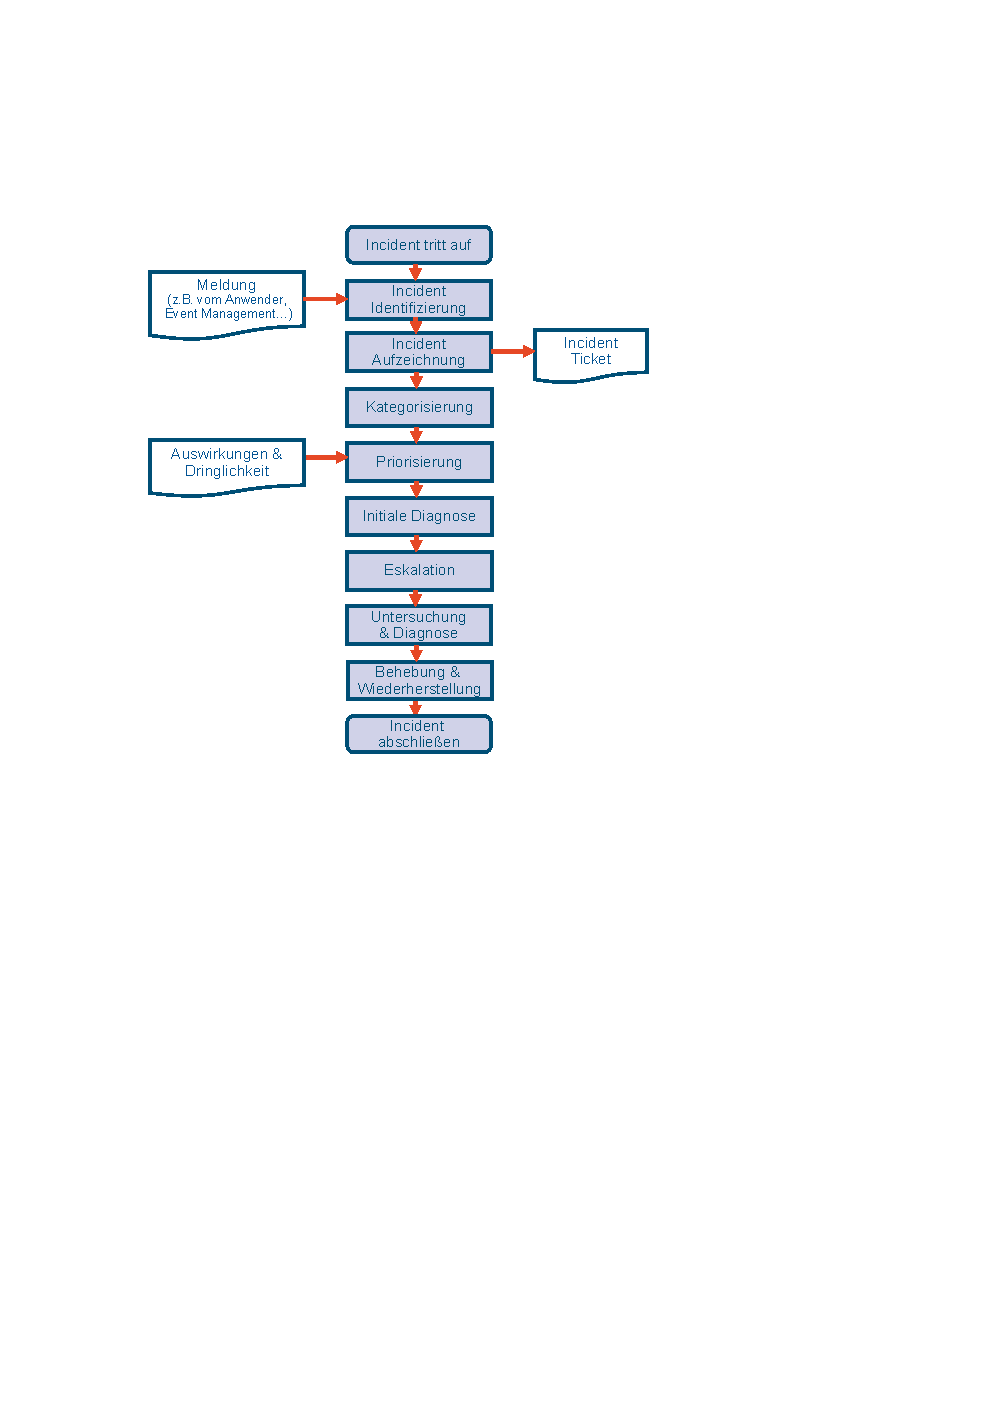
\includegraphics[width=0.7\linewidth]{fig/ablauf-incident-management}
\caption{Aktivitäten eines Incident Management Prozesses}
\label{fig:ablauf-incident-management}
\end{figure}

\subsubsection{Rollen}

\begin{description}
	\item[Incident Manager:] Der Incident Manager ist verantwortlich für einen funktionierenden Prozess und stellt sicher, dass die Aktivitäten innerhalb dieses Prozesses effektiv und effizient erfolgen.
	\item[1st Line Support:] Der 1st Line Support nimmt Anrufe entgegen und versucht Incidents mithilfe einer Knowledge Base zu lösen. Ungefähr 80\% aller Incidents können hier gelöst werden. Dauert die Bearbeitung aber länger als ca. eine halbe Stunde wird der Incident an den 2nd Line Support weitergegeben.
	\item[2nd Line Support:] Weitergeleitete Incidents werden von Spezialisten des IT-Betriebs behandelt. Der 2nd Line Support ist meisten nicht die Hauptaufgabe dieser Teams.
	\item[3rd Line Support:] Beim 3rd Line Support handelt es sich meist um externe Fachgruppen oder z.B. um einen Softwarehersteller der diesen Support anbietet.
\end{description}

\subsubsection{KPI's}

\begin{itemize}
	\item Durchschnittliche Kosten pro Incident
	\item Anteil falsch kategorisierter oder falsch zugewiesener Incidents
	\item Anzahl Major Incidents/Anzahl Incidents
\end{itemize}

\subsection{zwei ausgewählten IT-Betriebsprozesse der Testatübung:}

\subsubsection{Request Fulfilment}

\subsubsection{Ziele}

Das Request Fulfilment befasst sich mit dem Management von Anwenderfragen (z.B. Passwort zurücksetzen, Formel in Excel einfügen). Das Request Fulfilment sollte einen Kanal (keine Insellösungen) für den Bezug von Leistungen bereitstellen. Auch die Kommunikation und die Genehmigung der Leistungen müssen gewährleistet sein. Dadurch werden Prozesse wie Incident Management oder Change Management entlastet.

\subsubsection{Begriffe}

\begin{description}
	\item[Service Request:] Ein Service Request ist eine Anfrage eines Anwenders nach Informationen, Beratung oder Support.
	\item[Request Model:] Durch ein Request Model können ähnliche Requests effizient bearbeitet werden.
	\item[Menüauswahl:] Durch eine Menüauswahl kann der Anwender Standardleistungen aus einem Katalog auswählen und selbst beziehen.
	\item[Statusüberwachung:] Der Status jedes Request sollte über den gesamten Lifecycle verfolgt werden.
	\item[Request-Eskalation:] Man kann einen Request eskalieren lassen, um z.B. Probleme bei dessen Durchführung mit dem Change Management zu beseitigen.
	\item[Finanzielle Freigabe:] Die angeforderten Requests müssen auch bezahlt werden. Das stellt die finanzielle Freigabe sicher.
	\item[Weitere Freigaben:] Werden für einen Request z.B. zusätzliche Lizenzen benötigt braucht es weitere Freigaben.
	\item[Koordination der Ausführung:] Die meisten Request werden gleich vom Service-Desk Mitarbeiter erledigt. Sind jedoch weitere Schritte notwendig (z.B. Umzug durch Facility Management) müssen diese koordiniert werden.
\end{description}

\subsubsection{Aktivitäten}

\begin{description}
	\item[Request annehmen:] Ein Request wird über den Service Desk oder z.B. über eine automatische Bestellung entgegengenommen. Bei der Erfassung sollte zwischen einem Request und einem Incident unterschieden werden.
	\item[Logging und Validierung:] Alle Request müssen vollständig erfasst und mit einem Zeitstempel versehen werden.
	\item[Kategorisierung:] Für spätere Reports sollten Requests kategorisiert werden.
	\item[Priorisierung:] Die Requests werden im Zusammenhang mit dem Business priorisiert.
	\item[Autorisierung:] Bevor der Request ausgeführt wird muss überprüft werden ob der Benutzer diesen überhaupt ausführen darf.
	\item[Review:] Kann ein Request nicht alleine vom Service Desk bearbeitet werden, wird er weitergeleitet und die Durchführung überwacht.
	\item[Durchführung:] Der Request wird anhand eines Request Models durchgeführt.
	\item[Abschluss:] Nach der Bearbeitung des Requests wird er durch den Service Desk geschlossen.
\end{description}

\subsubsection{Rollen}

\begin{description}
	\item[Service-Desk-Mitarbeiter:] Sie nehmen die initiale Bearbeitung vor und führen einfache Service Requests direkt innerhalb des Service Desk durch.
	\item[Service-Operation-Teams:] Erfordern die Service Requests weitere Aktivitäten, wie z. B. die Lieferung oder den Umzug von Komponenten, werden diese von entsprechenden internen Teams oder beauftragten Dienstleistern durchgeführt.
	\item[Facility Management, Einkauf und weitere Abteilungen:] Sie werden bei der Erfüllung der Service Requests eingebunden und unterstützen bei Bedarf in Form der Übernahme von Aktivitäten oder Freigaben.
	\item[Dedizierte Support-Teams:] Werden eingesetzt wenn eine grosse Anzahl Requests ansteht oder kritische Anfragen vorliegen.
\end{description}

\subsubsection{KPI's}

\begin{itemize}
	\item Gesamtzahl der Service Requests
	\item Durchschnittliche Zeit für die Bearbeitung je Request Model
	\item Durchschnittliche Kosten für die Durchführung je Request Model
\end{itemize}

\subsubsection{Access Mgmt.}

\subsubsection{Ziele}

Das Access Management ist verantwortlich für die Verwaltung der Zugriffsrechte. Dazu muss ein Anwender identifiziert werden und dessen Zugriff geregelt werden. Dabei werden die Anweisungen des Security und Availability Management umgesetzt.

\subsubsection{Begriffe}

\begin{description}
	\item[Zugriff:] Der Begriff beschreibt das Niveau und Ausmaß der Befugnis eines Anwenders zur Nutzung eines Service und den Zugriff auf Daten.
	\item[Identität:] Die Identität eines Anwenders bezieht sich auf die Informationen und Eigenschaften, die ihn als Individuum ausweisen und seinen Status innerhalb der Organisation verifizieren.
	\item[Rechte:] Rechte beschreiben auf welche Services und Daten ein Anwender zugreifen darf.
	\item[Services oder Servicegruppen:] Die Vergabe von Rechten an Servicegruppen ist oft effizienter als die Vergabe von Rechten an einzelne Services.
\end{description}

\subsubsection{Aktivitäten}

\begin{description}
	\item[Zugriff anfordern:] Der Zugriff kann auf unterschiedliche Weise erfolgen z.B. über das Request Fulfilment.
	\item[Verifizierung:] Bevor die angeforderten Rechte vergeben werden können, wird zunächst die Identität des Anwenders verifiziert. Der Benutzer muss authentifiziert und überprüft werden ob er die Rechte erhalten darf.
	\item[Rechte vergeben:] In diesem Schritt wird autorisierten Benutzern der Zugriff auf entsprechende Services oder Daten gewährt. Das Access Management gewährt die Rechte aufgrund der Unternehmensanforderungen.
	\item[Überwachen des Identitätsstatus:] Der Status eines Mitarbeiters (z.B. Beförderung, Kündigung) muss ständig überwacht werden und die Rechte dementsprechend angepasst werden.
	\item[Protokollieren und Überwachen:] Das Access Management überwacht und protokolliert zusätzliche alle Zugriffe.
	\item[Rechte entfernen oder einschränken:] Ändert sich der Status eine Benutzer müssend die Rechte entfernt oder eingeschränkt werden.
\end{description}

\subsubsection{Rollen}

\begin{description}
	\item[Service Desk:] Der Service Desk nimmt die Anfragen entgegen, prüft sie gemäss den Vorgaben und Policies, richtet bei Bedarf die Berechtigungen ein und informiert den Antragsteller.
	\item[IT-Operations Management:] Das IT-Operations Management führt Ausbildungen und Trainings mit dem Service Desk durch.
\end{description}

\subsubsection{KPI's}

\begin{itemize}
	\item Anzahl der Anfragen zur Vergabe von Rechten
	\item Anzahl der Anpassungen aufgrund identifizierter Rollenänderungen
	\item Anzahl der Incidents aufgrund veränderter Berechtigungen
\end{itemize}
